\documentclass[rgb]{beamer}

\usepackage[english]{babel}
\usepackage[utf8]{inputenc}
\usepackage{xcolor}
\usepackage{listings}
\usepackage{adjustbox}
\usepackage{amsmath}
\usepackage{multirow}
\usepackage[linewidth=1pt]{mdframed}

% Graphics
\usepackage{graphicx}

\usepackage{tikz}
\usetikzlibrary{calc,shapes.multipart,chains,arrows}

% Font
\usepackage{paratype}
\setbeamerfont{frametitle}{family=\bf}

% Beamer theme settings
\usecolortheme{seagull}
\setbeamertemplate{itemize item}{\raisebox{0.8mm}{\rule{1.8mm}{1.2mm}}}
\usenavigationsymbolstemplate{} % no navigation buttons

\usepackage{listings}

% Define Language
\lstdefinelanguage{fsharp}
{
  % list of keywords
  morekeywords={
    and,
    do,
    else,
    exception,
    for,
    fun,
    function,
    if,
    in,
    let,
    match,
    module,
    mutable,
    open,
    of,
    rec,
    then,
    try,
    type,
    unsafe,
    use,
    val,
    when,
    while,
    with,
  },
  sensitive=true, % keywords are not case-sensitive
  morecomment=[l]{//}, % l is for line comment
%  otherkeywords={>,<,=,<=,>=,!,*,/,-,+,|,&,||,&&,==,=>},
  morestring=[b]" % defines that strings are enclosed in double quotes
}

% Define Colors
\usepackage{color}
\definecolor{eclipseBlue}{RGB}{42,0.0,255}
\definecolor{eclipseGreen}{RGB}{63,127,95}
\definecolor{eclipsePurple}{RGB}{127,0,85}

\newcommand{\fop}[1]{\mbox{\ttfamily\color{eclipseBlue}#1}}
\newcommand{\fw}[1]{\mbox{\ttfamily\bfseries\color{eclipsePurple}#1}}

% Set Language
\lstset{
  language={fsharp},
  basicstyle=\ttfamily, % Global Code Style
  captionpos=b, % Position of the Caption (t for top, b for bottom)
  extendedchars=true, % Allows 256 instead of 128 ASCII characters
  tabsize=2, % number of spaces indented when discovering a tab
  columns=fixed, % make all characters equal width
  keepspaces=true, % does not ignore spaces to fit width, convert tabs to spaces
  showstringspaces=false, % lets spaces in strings appear as real spaces
  breaklines=true, % wrap lines if they don't fit
  frame=trbl, % draw a frame at the top, right, left and bottom of the listing
  frameround=tttt, % make the frame round at all four corners
  framesep=4pt, % quarter circle size of the round corners
  numbers=left, % show line numbers at the left
  numberstyle=\small\ttfamily, % style of the line numbers
  commentstyle=\slshape\bfseries\color{eclipseGreen}, % style of comments
  keywordstyle=\bfseries\color{eclipsePurple}, % style of keywords
  stringstyle=\color{eclipseBlue}, % style of strings
  emph=[1] {
    false,
    true,
    Set,
    Map,
    List,
    ImgUtil,
    Pegs,
    String,
    Array,
    Array2D
  },
  emphstyle=[1]{\color{eclipseBlue}},
  moredelim=**[is][\color{red}]{@@}{@@}
}

\newcommand{\theyear}{2020}
\newcommand{\sem}[1]{[\![#1]\!]}
\newcommand{\seme}[1]{\sem{#1}\varepsilon}
\newcommand{\semzero}[1]{\sem{#1}_0}

\newcommand{\emptymap}{\{\}}
\newcommand{\fracc}[2]{\begin{eqnarray} \frac{\begin{array}{c} #1
    \end{array}}{\begin{array}{c} #2 \end{array}} \end{eqnarray}}
\newcommand{\sembox}[1]{\hfill \normalfont \mbox{\fbox{\(#1\)}}}
\newcommand{\sempart}[2]{\subsubsection*{\rm\em #1 \sembox{#2}}}
\newcommand{\axiom}[1]{\begin{eqnarray} \begin{array}{c} #1 \end{array} \end{eqnarray}}
\newcommand{\fraccn}[2]{\refstepcounter{equation}\mbox{$\frac{\begin{array}{c} #1 \end{array}}{\begin{array}{c} #2 \end{array}}$}~(\arabic{equation})}
\newcommand{\fraccc}[2]{\mbox{$\frac{\begin{array}{c} #1 \end{array}}{\begin{array}{c} #2 \end{array}}$}}
\newcommand{\onepart}[1]{\noindent\hfill#1\hfill~\vspace{2mm}}
\newcommand{\twopart}[2]{\noindent\hfill#1\hfill#2\hfill~\vspace{2mm}}
\newcommand{\threepart}[3]{\noindent\hfill#1\hfill#2\hfill#3\hfill~\vspace{2mm}}
%\newcommand{\axiomm}[1]{\refstepcounter{equation}\mbox{$\begin{array}{c} #1 \end{array}$}~(\arabic{equation})}
\newcommand{\axiomm}[1]{$\begin{array}{c} #1 \end{array}$}
%\newcommand{\ar}[1]{\stackrel{#1}{\longrightarrow}}
\newcommand{\vd}{\vdash}
\newcommand{\Ran}{{\rm Ran}}
\newcommand{\Dom}{{\rm Dom}}
\newcommand{\kw}[1]{\texttt{#1}}
\newcommand{\id}[1]{\mbox{\it{#1}}}
\newcommand{\rarr}{\rightarrow}
\newcommand{\eval}{\rarr}
\newcommand{\evals}{\leadsto}
\newcommand{\larr}{\leftarrow}

\newcommand{\head}[1]{\vspace{3mm} \textbf{\normalsize #1}}
\newcommand{\headsp}[1]{\head{#1}\vspace{1ex}}
\newcommand{\size}{\ensuremath{\mathrm{size}}}
\renewcommand{\log}{\ensuremath{\mathrm{log}}}

\newcommand{\setallthemecolors}[1]{%
\setbeamercolor*{palette primary}{use=structure,fg=white,bg=#1}%
\setbeamercolor*{palette secondary}{use=structure,fg=white,bg=#1}%
\setbeamercolor*{palette tertiary}{use=structure,fg=white,bg=#1}}

\definecolor{black}{RGB}{0,0,0}
\definecolor{maroon}{RGB}{128,0,0}
\definecolor{olive}{RGB}{128,128,0}
\definecolor{green}{RGB}{0,128,0}
\definecolor{purple}{RGB}{128,0,128}
\definecolor{teal}{RGB}{0,128,128}
\definecolor{darkteal}{RGB}{0,92,92}
\definecolor{navy}{RGB}{0,0,128}
\definecolor{gray}{RGB}{128,128,128}
\definecolor{darkgray}{RGB}{60,60,60}
\definecolor{darkred}{RGB}{139,0,0}

%palette

% #173F5F (dark blue)
\definecolor{darkblue}{RGB}{23,63,95}
% #20639B (blue)
\definecolor{blue}{RGB}{32,99,155}
% #3CAEA3 (green)
\definecolor{magenta}{RGB}{60,174,163}
% #F6D55C (yellow)
\definecolor{yellow}{RGB}{246,213,92}
% #ED553B (red)
\definecolor{red}{RGB}{237,85,59}


\usecolortheme{whale}
\useoutertheme{infolines}
\useinnertheme{rectangles}

\newcommand{\popsettitle}[2]{%
\setallthemecolors{#1}%
\newcommand{\popemne}{#2}%
\title{Programmering og Problemløsning}%
\subtitle{#2}%
\author{Martin Elsman}%
\date{}%
\institute[DIKU]{Datalogisk Institut, Københavns Universitet (DIKU)}}

\newcommand{\popmaketitleframe}{%
  \frame{\titlepage%
   \vspace{-15mm}%
   \par\noindent\rule{\textwidth}{0.4pt}%

   \vspace{4mm}%
   \tableofcontents%
   \vspace{-4mm}%
   \par\noindent\rule{\textwidth}{0.4pt}%
  }%
  \section*{\popemne}%
}


\popsettitle{olive}{Programmering med Lister (Del 2)}

\begin{document}

\popmaketitleframe

%%%%%%%%%%%%%%%%%%%%%%%%%%%%%%%%%%%%%%%%%%%%%%%%
\subsection{Tidligere om lister}
%%%%%%%%%%%%%%%%%%%%%%%%%%%%%%%%%%%%%%%%%%%%%%%%

\begin{frame}[fragile]
\headsp{Tidligere om lister...}
\begin{footnotesize}

\textbf{Syntax for lister}

\begin{lstlisting}[numbers=none,frame=none]
let nums = [1;2;3;4]                       // 1::2::3::4::[]
\end{lstlisting}

\textbf{Grundlæggende funktionalitet til konstruktion af lister}
\begin{lstlisting}[numbers=none,frame=none]
val []     : 'a list                       // empty list
val ::     : 'a -> 'a list -> 'a list      // add element
val @      : 'a list -> 'a list -> 'a list // append lists
\end{lstlisting}

\textbf{Lagerrepræsentation for lister}

\begin{lstlisting}[numbers=none,frame=none]
let lst = [1; 2; 3; 4]
let lst2 = 5 :: List.tail (List.tail lst)
\end{lstlisting}

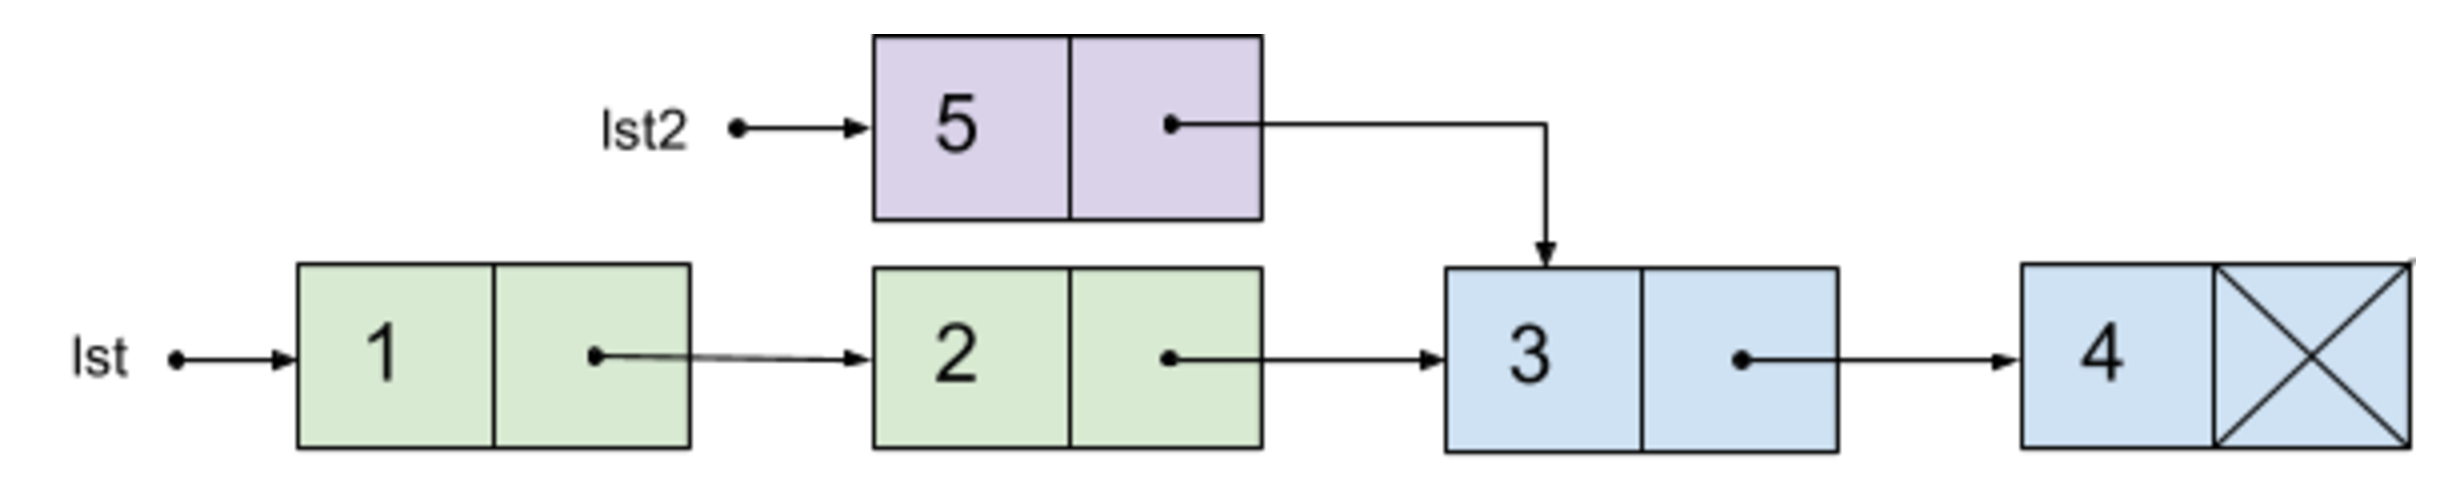
\includegraphics[width=.9\textwidth]{list1234.png}

\end{footnotesize}
\end{frame}

%%%%%%%%%%%%%%%%%%%%%%%%%%%%%%%%%%%%%%%%%%%%%%%%
\subsection{Modulet \lstinline{List}}
%%%%%%%%%%%%%%%%%%%%%%%%%%%%%%%%%%%%%%%%%%%%%%%%

\begin{frame}[fragile]
\begin{footnotesize}

\head{Modulet \lstinline{List}}

\vspace{1ex}

Modulet \lstinline{List} indeholder en lang række operationer på
lister.

\begin{lstlisting}[numbers=none]
// list creation
val init     : int -> (int -> 'a) -> 'a list

// list deconstruction
val head     : 'a list -> 'a
val tail     : 'a list -> 'a list

// list transformers
val map      : ('a -> 'b) -> 'a list -> 'b list
val map2     : ('a->'b->'c) -> 'a list -> 'b list -> 'c list
val filter   : ('a -> bool) -> 'a list -> 'a list
\end{lstlisting}

\begin{lstlisting}[numbers=none,frame=none]
// list traversing
val length   : 'a list -> int   // length l = l.Length
val fold     : ('s -> 'a -> 's) -> 's -> 'a list -> 's
val foldBack : ('a -> 's -> 's) -> 'a list -> 's -> 's
val find     : ('a -> bool) -> 'a list -> 'a option
...
\end{lstlisting}
\end{footnotesize}

\end{frame}

%%%%%%%%%%%%%%%%%%%%%%%%%%%%%%%%%%%%%%%%%%%%%%%%
\subsection{Dynamisk konstruktion af lister}
%%%%%%%%%%%%%%%%%%%%%%%%%%%%%%%%%%%%%%%%%%%%%%%%

\begin{frame}[fragile]
\begin{footnotesize}

  \head{Dynamisk konstruktion af lister}

  \vspace{1ex}

  Funktionen \lstinline{List.init} gør det muligt at opbygge en liste
  dynamisk fra bunden:

\begin{lstlisting}[numbers=none,frame=none,mathescape]
val init : int -> (int -> 'a) -> 'a list

 init $n$ f
   = [f $0$; f $1$; f $2$; ...; f $(n-1)$]
\end{lstlisting}

  \vspace{1ex}

  \head{Eksempel}

\begin{lstlisting}[numbers=none,frame=none,mathescape]
let sz = 2 + 3
let lst = List.init sz (fun x -> x * 2 + 1)

//  = [0*2+1; 1*2+1; 2*2+1; 3*2+1; 4*2+1]
// $\evals$  [1; 3; 5; 7; 9]
\end{lstlisting}

\end{footnotesize}
\end{frame}

%%%%%%%%%%%%%%%%%%%%%%%%%%%%%%%%%%%%%%%%%%%%%%%%
\subsection{Transformation af lister}
%%%%%%%%%%%%%%%%%%%%%%%%%%%%%%%%%%%%%%%%%%%%%%%%

\begin{frame}[fragile]
\begin{footnotesize}
  \head{Transformation af lister --- \lstinline{map} og \lstinline{map2}}
\vspace{0.5ex}

\begin{lstlisting}[numbers=none,frame=none,mathescape]
val map : ('a -> 'b) -> 'a list -> 'b list

 map f [v$_0$; v$_1$; v$_2$; ...; v$_n$]
   = [f v$_0$; f v$_1$; f v$_2$; ...; f v$_n$]

val map2 : ('a->'b->'c) -> 'a list -> 'b list -> 'c list

 map2 f [a$_0$; a$_1$; a$_2$; ...; a$_n$] [b$_0$; b$_1$; b$_2$; ...; b$_m$]
   = [f a$_0$ b$_0$; f a$_1$ b$_1$; f a$_2$ b$_2$; ...; f a$_n$ b$_n$]   // if n=m
   = ${\it runtime error}$                                // if n<>m
\end{lstlisting}

\head{Eksempler}
\vspace{0.5ex}
\begin{lstlisting}[numbers=none,frame=none,mathescape]
let vs = List.map (fun x -> x+1) [10; 20; 30]

//  = [10+1; 20+1; 30+1]  $\evals$  [11; 21; 31]

let us = List.map2 (+) [10; 20; 30] [1; 2; 3]

//  = [10+1; 20+2; 30+3]  $\evals$  [11; 22; 33]
\end{lstlisting}

\end{footnotesize}
\end{frame}

\begin{frame}[fragile]
\begin{footnotesize}

\head{Transformation af lister --- \lstinline{List.filter}}
\vspace{1ex}

\begin{lstlisting}[numbers=none,frame=none,mathescape]
val filter : ('a -> bool) -> 'a list -> 'a list
\end{lstlisting}

\vspace{1ex}

Udtrykket (\lstinline{List.filter p xs}) resulterer i en liste
indeholdende de elementer i \lstinline{xs} der opfylder prædikatet
\lstinline{p}.

\vspace{1ex}
\head{Eksempel}
\vspace{1ex}
\begin{lstlisting}[numbers=none,frame=none,mathescape]
let allcaps = [("London",8.8); ("Berlin",3.5);
               ("Copenhagen",0.7); ("New York",8.5);
               ("Rome",2.9)]
let bigcaps = List.filter (fun (name,sz) -> sz > 5.0) allcaps

// $\evals$ [("London",8.8);("New York",8.5)]
\end{lstlisting}

\end{footnotesize}
\end{frame}

\subsection*{Konklusion}
\begin{frame}[fragile]
  \headsp{Konklusion}

  \vspace{3mm}
  \tableofcontents
\end{frame}

\end{document}
